\chapter{冰川模式}
\begin{mymdframed}{代码}
    本节对应的代码文件为\texttt{MOD\_Glacier.F90}。
\end{mymdframed}
\section{冰川模式结构}
冰川模式的结构类似于雪盖土壤层,区别在于冰川模式将土壤层替换为了冰层。即在CoLM中,冰川分为上部的雪盖层和下部的冰川冰层(图~\ref{fig:模式中雪盖土壤和雪盖冰川的分层对比})。雪盖根据雪盖高度$z_{sno}$被分为最多五层,这种情况下,雪层从上到下分别用$i=-4,-3,-2,-1,0$编号。$i=0$表示底层,与冰面相邻,$i=snl+1$表示顶层,$snl$表示雪层总数的负数($-5\leqslant snl\leqslant 0$)。冰川冰的分层规则和土壤一致,默认分为10层,具体分层规则见章节~\ref{土壤和积雪的垂直分层}。雪盖冰川层的厚度表示为$\Delta z_i$(m),每一层的深度$z_i$(m)取为其上边界深度 $z_{h,i-1}$和下边界深度$z_{h,i}$的中点。冰川模式的物理方案均遵从无植被覆盖下的雪盖土壤层的计算方案来设定。

 {
\begin{figure}[htbp]
\centering
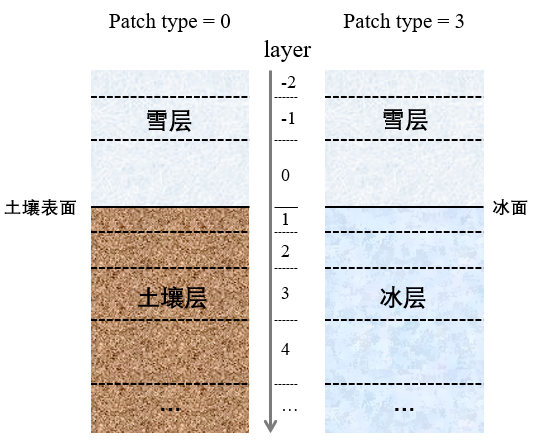
\includegraphics[width=0.8\textwidth]{Figures/冰川模式/模式中雪盖土壤和雪盖冰川的分层对比.jpg}
\caption{模式中雪盖土壤和雪盖冰川的分层对比}
\label{fig:模式中雪盖土壤和雪盖冰川的分层对比}
\end{figure}
}

\section{冰川表面湍流通量计算方案}
冰川表面湍流通量的计算方案类似无植被覆盖下的雪盖土壤地表的湍流通量计算方案(见章节~\ref{无植被覆盖地表湍流通量的计算方案}),这里再对计算流程做一个简单说明。

冰川表面可以分为被积雪覆盖和未被积雪覆盖两部分,因此在计算湍流通量前,需先计算地表的积雪覆盖比例$f_{sno}$,根据~\citet{swenson2012new},$f_{sno}$的计算包含以下两个过程:

1.在积分开始时,若发生降雪,则下一时间步数的$f_{sno}$更新为
\begin{equation}
    f^{n+1}_{sno}=1-\left[1-\tanh{\left(0.1 p_i \Delta t\right)}\right]\left(1-f^n_{sno}\right) \leqslant 1.0
\end{equation}
其中$p_i$表示到达冰川表面的固态降水率(\unit{kg.m^{-2}.s^{-1}}),$\Delta t$为积分的时间步长(s);

2.在水热过程模拟结束后,考虑积雪融化,$f_{sno}$更新为
\begin{equation}
    f^{n+1}_{sno}=\tanh \left(\frac{100 z^2_{sno}}{2.5z_{0m,ice} W_{sno}}\right)
\end{equation}
其中$z_{sno}$为雪盖高度(mm),$W_{sno}$为雪水当量(mm),$z_{0m,ice}$表示未被积雪覆盖时冰川的地表粗糙度(目前与裸土相同,取为0.01)。


由于冰川属于无植被覆盖的陆地表面,因此湍流通量只存在于地表和大气之间,动量通量$\tau$、感热通量$H$和水汽通量$E$分别表达为:
\begin{align}
    \tau_x &= -\rho_{atm} \frac{u_{atm}}{r_{am}} \\
    \tau_y &= -\rho_{atm} \frac{v_{atm}}{r_{am}} \\
    H_g &= -\rho_{atm} C_{pa} \frac{\theta_{atm}-T_g}{r_{ah}} \\
    E_g &= -\rho_{atm} \frac{q_{atm}-q_g}{r_{aw}}
\end{align}
其中$\rho_{atm}$表示空气密度(\unit{kg.m^{-3}}),$u_{atm}$和$v_{atm}$分别表示纬向风速和经向风速,$C_{pa}$表示空气的比热容(\unit{J.kg^{-1}.K^{-1}}),$\theta_{atm}$表示大气位温(K),$r_{am}$、$r_{ah}$和$r_{aw}$分别表示空气动力学、感热通量和水汽通量的湍流阻抗系数(\unit{s.m^{-1}}),$T_g$表示地表温度(K),当有积雪覆盖时,$T_g$为最上层雪层的温度,否则,$T_g$取为第一层冰层的温度。$q_g$表示地表空气的比湿,取为温度在$T_g$时的饱和比湿,即$q_g=q^{T_g}_{sat}$。

由于地表无植被覆盖,在计算阻抗系数$r_{am}$、$r_{ah}$、$r_{aw}$时,零平面位移取为$d=0$。动量粗糙度在无积雪覆盖时取为$z_{0m}=0.001$,有积雪覆盖时取为$z_{0m}=0.002$ \citep{brock_willis_sharp_2006}。感热和水汽粗糙度取为:
\begin{equation}z_{0h}=z_{0w}=z_{0m}\exp{\left[-0.13\left(Re_*\right)^{0.45}\right]}
\end{equation}
其中$Re_*=u_*\cdot z_{0m}/v$表示粗糙雷诺数,$v= 1.5 \times 10^{-5}$ \unit{m^2.s^{-1}}为空气动力学粘性系数。

基于此,冰川表面湍流通量的具体计算流程如下:
\begin{enumerate}
    \item 给出计算风速$V_a$时$U_c$的初始猜测:
        \begin{equation}
            U_c = \begin{cases}
                0, &\text{当}\ \theta_{v_atm}-\theta_{v,s} \geqslant 0 \text{ 时(稳定条件)} \\
                0.5, &\text{当}\ \theta_{v_atm}-\theta_{v,s} < 0 \text{ 时(不稳定条件)}
            \end{cases}
        \end{equation}
    \item 通过$R_{ib}$给出Monin-Obukhov长度$L$的初始猜测;
    \item 迭代以下过程以获得冰川表面的能量通量:\\
        a. 通过风速、温度和比湿的微风方程积分结果求解$u_*$、$\theta_*$和$q_*$,\\
        b. 更新感热和水汽粗糙度$z_{0h}$和$z_{0w}$,\\
        c. 计算虚位温尺度$\theta_{v*}$,\\
        d. 更新大气风速$V_a$,\\
        e. 计算新一步$L$,\\
        每完成上面的一次迭代过程判断$L$是否改变符号,若符号改变达到四次或以上,视为中性条件,跳出迭代,否则持续迭代直至6次;
    \item 计算湍流阻抗系数$r_{am}$、$r_{ah}$和$R_{aw}$;
    \item 计算动量通量$\tau_x$、$\tau_y$,感热通量$H_g$和水汽通量$E_g$;
    \item 计算 2-m气温$T_{2m}$和比湿$q_{2m}$。
\end{enumerate}

\section{冰川温度计算方案}
冰川垂直层温度的计算方案同样类似于雪盖土壤层的垂直层温度计算方案。假设冰川无水平物质能量交换,则垂直方向上的一维能量平衡方程如下:
\begin{equation}\label{eq:GlacierThermalCons}
    c \frac{\partial T}{\partial t}=-\frac{\partial F}{\partial z},  \quad F=-\lambda \frac{\partial T}{\partial z}
\end{equation}
其中$c$表示雪盖或冰川冰的体积热容(\unit{J.m^{-3}.K^{-1}}),$T$表示雪盖或冰川冰温度(K),$t$表示时间(s),$z$表示雪盖冰川层的深度,$F$表示垂直方向的热通量(向上为正方向,\unit{W.m^{-2}}),$\lambda$表示热导率(\unit{W.m^{-1}.K^{-1}})。由于冰川仅考虑由液态水和固态水组成,其体积热容和热导率计算与其它雪盖土壤层稍有不同,采用简化的计算方案,下面详细说明。

对于体积热容,其由每层液态水和固态水的体积热容根据各自体积百分比加权得到,即
\begin{equation}
    c_i = \frac{w_{ice,i}}{\Delta z_i}C_{pi} + \frac{w_{liq,i}}{\Delta z_i}C_{pl}
\end{equation}
其中,$w_{ice,i}$和$w_{liq,i}$分别表示第$i$层固态水含量和液态水含量(\unit{kg.m^{-2}}),$C_{pl}$和$C_{pi}$分别表示固态水和液态水的体积热容量(见表~\ref{tab:物理常数})。特别地,若此时无雪盖分层但雪水当量$W_{sno}>0$,则将这部分热容量考虑为固态水的热容量加到冰层顶层中,冰层顶层(即编号$i=1$)热容量重新计算为:
\begin{equation}
    c_1 = \frac{w_{ice,1}+W_{sno}}{\Delta z_1}C_{pi} + \frac{w_{liq,1}}{\Delta z_1}C_{pl}
\end{equation}

对于热导率,雪层部分(即$snl+1\leqslant i\leqslant 0$)采用~\citet{jordan1991one}提出的方案:
\begin{equation}
    \lambda_i = \lambda_a + \left(7.75 \times 10^{-5} \rho_{sno,i} + 1.105\times 10^{-6} \rho^2_{sno,i}\right)\left(\lambda_{ice}-\lambda_a\right)
\end{equation}
其中$\lambda_a$表示空气的热导率(\unit{W.m^{-1}.K^{-1}}),$\rho_{sno,i}=\left(w_{liq,i}+w_{ice,i}\right)/\Delta z_i$表示第$i$层雪层的平均密度(\unit{kg.m^{-3}}),$\lambda_{ice}$为固态水的热导率(表A.1)。冰层部分(即$1\leqslant i \leqslant 10$)采用~\citet{yen1981review}提出的方案:
\begin{equation}
    \lambda_i =\begin{cases}
        \lambda_{liq} &\text{当}\ T_i > T_f \text{ 时} \\
        9.828 e^{-0.0057 T_i} &\text{当}\ T_i \leqslant T_f \text{ 时}
    \end{cases}
\end{equation}
其中$\lambda_{liq}$为液态水的热导率(表~\ref{tab:物理常数})

对方程~\eqref{eq:GlacierThermalCons} 进行离散(见章节~\ref{温度求解的数值格式}),则第$i$层雪盖冰川层的能量平衡方程可表达为:
\begin{equation}\label{eq:GlacierThermal}
    \frac{c_i \Delta z_i}{\Delta t} \left(T^{n+1}_i - T^n_i\right) = F_i - F_{i-1}
\end{equation}
其中$\Delta t$表示积分时间步长,$n$表示时间步数,$F_i$表示第$i+1$层传导到第$i$层的热通量,其离散形式为:
\begin{equation}
    F_i = \lambda \left[z_{h,i}\right] \frac{T_i-T_{i+1}}{z_i-z_{i+1}}
\end{equation}
$\lambda\left[z_{h,i}\right]$表示第$i+1$层和第$i$层交界面处的热导率:
\begin{equation}
    \lambda \left[z_{h,i}\right] = \begin{cases}
        \frac{\lambda_i\lambda_{i+1}\left(z_i-z_{i-1}\right)}{\lambda_i\left(z_{h,i}-z_{i+1}\right)+\lambda_{i+1}\left(z_i-z_{h,i}\right)}  &\text{对于}\ i=snl+1,\ \ldots,\ 9 \\
        0 &\text{对于}\ i=10
    \end{cases}
\end{equation}
特别的,对于雪盖与冰川冰的交界面,为防止最下层雪层厚度过大导致$\lambda\left[z_{h,i}\right]$计算不准,当$i=0$且$z_{i+1}-z_{h,i}<z_{h,i}-z_i$时,该处的$\lambda\left[z_{h,0}\right]$重新计算为:
\begin{equation}
    \lambda\left[z_{h,0}\right]=\frac{2\lambda_0\lambda_1}{\lambda_0+\lambda_1} \geqslant 0.5\lambda_1
\end{equation}

对方程~\eqref{eq:GlacierThermal}采用Crank-Nicholson半隐式格式求解,得到以下形式:
\begin{equation}
    \frac{c_i\Delta z_i}{\Delta t}\left(T^{n+1}_i - T^n_i\right)=\alpha \left(F^n_i - F^n_{i-1}\right) + \left(1-\alpha \right) \left(F^{n+1}_i - F^{n+1}_{i-1}\right)
\end{equation}
其中$\alpha = 0.5$为权重因子。将所有雪盖冰川层的能量平衡方程联立,得到三对角矩阵形式的方程组:
\begin{equation}
    r_i = a_i T^{n+1}_{i-1} + b_i T^{n+1}_i + c_i T^{n+1}_{i+1}
\end{equation}
其中$a_i$,$b_i$和$c_i$分别为三对角矩阵中上三角、对角线和下三角位置中的元素。下面分别阐述不同情况下三对角矩阵中系数的具体表达。

(1)对于冰川的中间层(即$snl+1<i<10$),三对角矩阵中的系数表达如下
\begin{equation}
    \begin{aligned}
        a_i &= -\left(1-\alpha \right) \frac{\Delta t}{c_i \Delta z_i} \frac{\lambda \left[z_{h,i-1}\right]}{z_i-z_{i-1}} \\
        b_i &= 1+\left(1-\alpha \right) \frac{\Delta t}{c_i \Delta z_i} \left[\frac{\lambda \left[z_{h,i-1}\right]}{z_i-z_{i-1}} + \frac{\lambda \left[z_{h,i}\right]}{z_{i+1}-z_i}\right] \\
        c_i &= -\left(1-\alpha \right)\frac{\Delta t}{c_i\Delta z_i}\frac{\lambda \left[z_{h,i}\right]}{z_{i+1}-z_i} \\
        r_i &= T_{i}^{n}+\alpha \frac{\Delta t}{c_{i} \Delta z_{i}} \lambda\left[z_{h, i}\right] \frac{T_{i}^{n}-T_{i+1}^{n}}{z_{i}-z_{i+1}}-\lambda\left[z_{h, i-1}\right] \frac{T_{i-1}^{n}-T_{i}^{n}}{z_{i-1}-z_{i}}
    \end{aligned}
\end{equation}

(2)对于冰川顶层(即$i=snl+1$),其向上的热通量即为大气进入到地表的热通量$h_s$
\begin{equation}
    h^{n+1}_s=-\alpha F^n_{i-1}-\left(1-\alpha\right)F^{n+1}_{i-1}
\end{equation}
此时顶层的能量平衡方程为:
\begin{equation}
    \frac{c_i\Delta z_i}{\Delta t}\left(T^{n+1}_i-T^n_i\right) = h^{n+1}_s+\alpha F^n_i+\left(1-\alpha \right)F^{n+1}_{i-1}
\end{equation}
其中$h^{n+1}_s$取一阶泰勒近似:
\begin{equation}
    h^{n+1}_s \approx h^n_s + \frac{\partial h_s}{\partial T_i}\left(T^{n+1}_i-T^n_i\right)
\end{equation}
于是,冰川顶层的三对角矩阵系数即为:
\begin{equation}
\begin{aligned}
    a_{i} &= 0 \\ 
    b_{i} &= 1+\frac{\Delta t}{c_{i} \Delta z_{i}}\left[(1-\alpha) \frac{\lambda\left[z_{h, i}\right]}{z_{i+1}-z_{i}}-\frac{\partial h_{s}}{\partial T_{i}}\right] \\
    c_{i} &= -(1-\alpha) \frac{\Delta t}{c_{i} \Delta z_{i}} \frac{\lambda\left[z_{h, i}\right]}{z_{i+1}-z_{i}} \\
    r_{i} &= T_{i}^{n}+\frac{\Delta t}{c_{i} \Delta z_{i}}\left[h_{s}^{n}-\frac{\partial h_{s}}{\partial T_{i}} T_{i}^{n}+\alpha \lambda\left[z_{h, i}\right] \frac{T_{i}^{n}-T_{i+1}^{n}}{z_{i}-z_{i+1}}\right]
\end{aligned}
\end{equation}

大气进入地表的热通量$h_s$和其偏导可计算为:
\begin{equation}\label{eq:GlacierSrfEnergyBalance}
    h_s = S_g + L_g - H_g - \lambda E_g + H_{prcg}
\end{equation}
\begin{equation}
    \frac{\partial h_s}{\partial T} = \frac{\partial L_g}{\partial T} -\frac{\partial H_g}{\partial T} -\frac{\partial \lambda E_g}{\partial T} +\frac{\partial H_{prcg}}{\partial T}
\end{equation}
其中$S_g$和$L_g$分别表示地表吸收的净太阳辐射和净长波辐射(\unit{W.m^{-2}}),$H_g$和$E_g$分别表示地表向大气输送的感热通量(\unit{W.m^{-2}})和水汽通量(\unit{kg.m^{-2}}),$H_{prcg}$表示降水与地表的能量交换
\begin{equation}
    H_{prcg} = C_{pl}p_l\left(T_p-T_g\right) + C_{pi}p_i\left(T_p-T_g\right)
\end{equation}
其中$p_l$和$p_i$分别表示到达地面的液态降水和固态降水(\unit{mm.H_2O.s^{-1}}),$T_p$表示降水温度(K)。
式~\eqref{eq:GlacierSrfEnergyBalance} 中$\lambda$表示潜热通量系数,用于将水汽通量转换为潜热通量
\begin{equation}
    \lambda = \begin{cases}
        \lambda_s &\text{当}\ w_{liq,snl+1}=0\text{ 且}\ w_{ice,snl+1}>0\text{ 时}\\
        \lambda_v &\text{当}\ w_{liq,snl+1}>0\text{ 时}
    \end{cases}
\end{equation}
$\lambda_s$和$\lambda_v$分别为固态水升华潜热系数和液态水蒸发潜热系数(表~\ref{tab:物理常数})。

对于式~\eqref{eq:GlacierSrfEnergyBalance} 中的净长波辐射$L_g$,其可计算为
\begin{equation}
    L_g = \varepsilon_g L_{bg}\downarrow - L_g\uparrow
\end{equation}
其中$L_{bg}\downarrow$表示近地面大气下行长波辐射,$L_g\uparrow=\varepsilon_g\sigma T^4_g$表示冰川表面发出的上行长波辐射,$\varepsilon_g=0.97$表示冰川表面的长波辐射发射率,$\sigma$表示Stefan-Boltzmann常数(表~\ref{tab:物理常数})。

另外,为改进由于冰川表面温度取为冰川顶层的平均温度带来的缺陷,在求解第一层能量平衡方程时,其厚度$\Delta z_i$调整为:
\begin{equation}
    \Delta z_i = 0.5\left[z_i-z_{h,i-1}+c_a\left(z_{i+1}-z_{h,i-1}\right)\right]
\end{equation}
其中调整参数取为$c_a=0.34$。

(3)对于冰川底层(即$i=10$),假定向下的热通量为0,则能量平衡方程变为:
\begin{equation}
    \frac{c_{i} \Delta z_{i}}{\Delta t}\left(T_{i}^{n+1}-T_{i}^{n}\right)=-\alpha \lambda\left[z_{h, i-1}\right] \frac{T_{i-1}^{n}-T_{i}^{n}}{z_{i-1}-z_{i}}-(1-\alpha) \lambda\left[z_{h, i-1}\right] \frac{T_{i-1}^{n+1}-T_{i}^{n+1}}{z_{i-1}-z_{i}}
\end{equation}
此时的三对角矩阵系数为:
\begin{equation}
\begin{aligned}
a_{i} &= -(1-\alpha) \frac{\Delta t}{c_{i} \Delta z_{i}} \frac{\lambda\left[z_{h, i-1}\right]}{z_{i}-z_{i-1}} \\
b_{i} &= 1+(1-\alpha) \frac{\Delta t}{c_{i} \Delta z_{i}} \frac{\lambda\left[z_{h, i-1}\right]}{z_{i}-z_{i-1}} \\
c_{i} &= 0 \\
r_{i} &= T_{i}^{n}-\alpha \frac{\Delta t \lambda\left[z_{h, i-1}\right]}{c_{i} \Delta z_{i}} \frac{T_{i-1}^{n}-T_{i}^{n}}{z_{i-1}-z_{i}}
\end{aligned}
\end{equation}

于是,通过求解上述的能量平衡方程组,即可计算出下一时刻的雪盖冰川层温度。之后,需再根据水的相态变化对温度进一步调整。冰川温度的相态变化调整与雪盖土壤部分完全一致,读者可参见章节\ref{sec:温度的相态变化调整}。至此,已完成冰川温度计算的全部过程,在得到$T^{n+1}_i$后,冰川表面发出的上行长波辐射$L_g\uparrow$、感热通量$H_g$与潜热通量$\lambda E_g$需做一次更新以作为输出的状态变量,其中用于蒸发的水汽不能超过冰川顶层的总水含量$\left(w^{n+1}_{liq,snl+1}+w^{n+1}_{ice,snl+1}\right)/\Delta t$,否则将顶层的总水含量用于蒸发,并将多余的能量误差加到感热通量上。


\section{冰川的水文过程计算方案}
在CoLM的冰川系统中,冰层的厚度与质量始终固定不变,故水文过程主要发生在冰层之上的雪盖层。采用这种处理方法的原因是,冰川通常位于水的冻结温度以下,CoLM假定冰层的融水会滞留在原地等待重新冻结,即使在较为温暖的一些区域,冰层融化的液态水也被认为永久滞留在冰层之中,不与外界进行水通量的交换。

对于仅需考虑的雪盖水文过程,按以下流程进行计算,其中每个部分在前文均有完整介绍,读者可自行翻阅。
\begin{enumerate}
    \item 计算雪盖垂直方向的液态水通量,并更新下一积分步数每一层的液态水含量,由雪盖底层流出的液态水通量则用于地表径流的计算当中(章节~\ref{雪盖的水量平衡});
    \item 考虑积雪的压实过程,更新每一层雪盖的厚度(章节~\ref{雪的压实});
    \item 当雪层发生消融至固态水含量过低或不足规定的最小厚度时,对雪层进行合并(章节~\ref{雪层的合并});当雪层积累至规定的最大厚度时,对雪层进行再分层(章节~\ref{雪层的再分层})。
\end{enumerate}

特别的,若冰川表面无雪盖存在,则冰层顶层(即$i=1$)的液态水和固态水含量根据下式更新:
\begin{equation}
    \begin{aligned}
        w^{n+1}_{liq,1} &= w^{n}_{liq,1} + q_{sdew} \Delta t \\
        w^{n+1}_{ice,i} &= w^{n}_{ice,1} + \left(q_{frost}-q_{subl}\right) \Delta t
    \end{aligned}
\end{equation}
其中$q_{sdew}$、$q_{frost}$和$q_{subl}$分别表示水的凝结、凝华和升华速率(\unit{kg.m^{-2}.s^{-1}}或\unit{mm.H_2O.s^{-1}})。
